\documentclass{minimal}
\usepackage{lmodern}
\usepackage{tikz}
\usetikzlibrary{arrows.meta,calc,positioning}
\usepackage{xcolor}

\definecolor{ink}{HTML}{17202A}
\definecolor{muted}{HTML}{5C6670}
\definecolor{paper}{HTML}{FCFDFE}
\definecolor{blue}{HTML}{2F6F9F}
\definecolor{bluefill}{HTML}{E7F0F7}
\definecolor{green}{HTML}{287B61}
\definecolor{greenfill}{HTML}{E3F2EC}
\definecolor{purple}{HTML}{66559B}
\definecolor{purplefill}{HTML}{ECE8F5}
\definecolor{orange}{HTML}{B5661D}
\definecolor{orangefill}{HTML}{F9EAD8}
\definecolor{grayfill}{HTML}{F0F2F4}

\pdfpagewidth=1000pt
\pdfpageheight=370pt
\setlength{\paperwidth}{1000pt}
\setlength{\paperheight}{370pt}
\setlength{\textwidth}{1000pt}
\setlength{\textheight}{370pt}
\setlength{\oddsidemargin}{-72pt}
\setlength{\topmargin}{-72pt}
\setlength{\headheight}{0pt}
\setlength{\headsep}{0pt}
\setlength{\footskip}{0pt}
\setlength{\parindent}{0pt}
\pagestyle{empty}

\begin{document}
\begin{tikzpicture}[
  x=1pt,y=1pt,
  font=\sffamily,
  line cap=round,
  line join=round,
  inference/.style={-{Latex[length=9pt,width=6pt]},draw=ink,line width=2.2pt},
  supervision/.style={-{Latex[length=9pt,width=6pt]},draw=orange,
                      densely dashed,line width=2.0pt},
  intervention/.style={-{Latex[length=8pt,width=5pt]},draw=muted,
                       densely dotted,line width=2.0pt},
  module/.style={rounded corners=8pt,draw=ink,line width=1.6pt,
                 fill=paper,align=center,minimum height=48pt},
  input/.style={module,fill=bluefill},
  state/.style={module,fill=greenfill},
  transition/.style={module,fill=purplefill},
  closure/.style={module,fill=orangefill},
  condition/.style={rounded corners=9pt,draw=purple,line width=1.3pt,
                    fill=paper,minimum height=24pt,align=center},
  evidence/.style={rounded corners=9pt,draw=ink!55,line width=1.4pt,
                   fill=paper,align=left,minimum width=284pt,minimum height=57pt},
  optional/.style={evidence,draw=muted,densely dashed,fill=grayfill}
]
\useasboundingbox (0,0) rectangle (1000,370);
\fill[paper] (0,0) rectangle (1000,370);

% Column headings and legend.
\node[anchor=west,text=ink,font=\sffamily\bfseries\fontsize{20}{23}\selectfont]
  at (22,350) {TerraState: predictive state in the forecast closure};
\node[anchor=west,text=ink,font=\sffamily\bfseries\fontsize{17}{20}\selectfont]
  at (700,350) {Matched verification};
\draw[ink!20,line width=1pt] (22,334) -- (978,334);
\draw[ink!20,line width=1pt] (675,18) -- (675,326);

\draw[inference] (25,316) -- (72,316);
\node[anchor=west,text=muted,font=\sffamily\fontsize{15}{18}\selectfont]
  at (80,316) {inference};
\draw[supervision] (176,316) -- (223,316);
\node[anchor=west,text=muted,font=\sffamily\fontsize{15}{18}\selectfont]
  at (231,316) {training supervision};
\draw[intervention] (420,316) -- (467,316);
\node[anchor=west,text=muted,font=\sffamily\fontsize{15}{18}\selectfont]
  at (475,316) {post-training test};

% Inference path.
\node[input,minimum width=110pt,font=\sffamily\bfseries\fontsize{17}{20}\selectfont]
  (history) at (76,250) {cloud-masked\\EO history};
\node[input,minimum width=74pt,font=\sffamily\bfseries\fontsize{19}{22}\selectfont]
  (q) at (194,250) {$q_{\theta,\rho}$};
\node[state,minimum width=92pt,font=\sffamily\bfseries\fontsize{19}{22}\selectfont]
  (zt) at (312,250) {$z_t$};
\node[transition,minimum width=112pt,font=\sffamily\bfseries\fontsize{18}{21}\selectfont]
  (trans) at (458,250) {shared $T_\psi$};
\node[state,minimum width=100pt,font=\sffamily\bfseries\fontsize{19}{22}\selectfont]
  (zh) at (602,250) {$z_{t+h}$};

\draw[inference] (history.east) -- (q.west);
\draw[inference] (q.east) -- (zt.west);
\draw[inference] (zt.east) -- (trans.west);
\draw[inference] (trans.east) -- (zh.west);

\node[condition,minimum width=150pt,font=\sffamily\bfseries\fontsize{15}{18}\selectfont]
  (contextaux) at (194,292) {past met. + static $g$};
\node[condition,minimum width=105pt,font=\sffamily\bfseries\fontsize{15}{18}\selectfont]
  (weather) at (377,292) {full24 future};
\node[condition,minimum width=78pt,font=\sffamily\bfseries\fontsize{15}{18}\selectfont]
  (transgeo) at (480,292) {static $g$};
\node[condition,minimum width=82pt,font=\sffamily\bfseries\fontsize{15}{18}\selectfont]
  (horizon) at (574,292) {horizon $h$};
\draw[inference,line width=1.5pt] (contextaux.south) -- (q.north);
\draw[inference,line width=1.5pt] (weather.south) -- ($(trans.north)+(-35pt,0)$);
\draw[inference,line width=1.5pt] (transgeo.south) -- (trans.north);
\draw[inference,line width=1.5pt] (horizon.south) -- ($(trans.north)+(35pt,0)$);

% Explicit closure: prior and state contribution meet at addition.
\node[input,minimum width=118pt,font=\sffamily\bfseries\fontsize{17}{20}\selectfont]
  (prior) at (352,173) {context prior\\$b_h$};
\node[closure,minimum width=112pt,font=\sffamily\bfseries\fontsize{17}{20}\selectfont]
  (odecode) at (430,111) {$O_\omega(z_{t+h})$};
\node[circle,draw=ink,line width=1.8pt,fill=paper,minimum size=39pt,
      font=\sffamily\bfseries\fontsize{24}{27}\selectfont]
  (plus) at (531,145) {$+$};
\node[closure,minimum width=92pt,font=\sffamily\bfseries\fontsize{16}{19}\selectfont]
  (pred) at (618,145) {prediction\\$\widehat y_{t+h}$};

\draw[inference] (q.south) |- (prior.west);
\draw[inference] (zh.south) -- (odecode.north);
\draw[inference] (prior.east) -- (plus.north west);
\draw[inference] (odecode.east) -- (plus.south west);
\draw[inference] (plus.east) -- (pred.west);

% Training-only future-state anchor.
\node[input,draw=orange,fill=orangefill,minimum width=130pt,
      font=\sffamily\bfseries\fontsize{16}{19}\selectfont]
  (futureeo) at (82,67) {observed future EO};
\node[module,draw=orange,minimum width=130pt,
      font=\sffamily\bfseries\fontsize{16}{19}\selectfont]
  (targetenc) at (259,67) {frozen $q/P_\rho$};
\node[state,draw=orange,minimum width=96pt,
      font=\sffamily\bfseries\fontsize{18}{21}\selectfont]
  (zstar) at (413,67) {$z^\star_{t+20}$};
\node[closure,draw=orange,minimum width=124pt,
      font=\sffamily\bfseries\fontsize{16}{19}\selectfont]
  (align) at (588,67) {future-state\\alignment};

\draw[supervision] (futureeo.east) -- (targetenc.west);
\draw[supervision] (targetenc.east) -- (zstar.west);
\draw[supervision] (zstar.east) -- (align.west);
\draw[supervision] (zh.east) -- ++(12pt,0) |- (align.east);

% Evidence panels: Q1--Q3 core, Q4 visually secondary.
\node[evidence,anchor=north west,font=\sffamily\fontsize{16}{19}\selectfont]
  (q1) at (695,318) {\textbf{\color{blue}Q1 Forecast skill}\\
                     \hspace{5pt}same selected checkpoint};
\node[evidence,anchor=north west,font=\sffamily\fontsize{16}{19}\selectfont]
  (q2) at (695,247) {\textbf{\color{blue}Q2 Load-bearing}\\
                     \hspace{5pt}full \quad closure cut \quad $T\!\to\!I$};
\node[evidence,anchor=north west,font=\sffamily\fontsize{16}{19}\selectfont]
  (q3) at (695,176) {\textbf{\color{green}Q3 Driver response}\\
                     \hspace{5pt}matched \quad mean \quad donor};
\node[optional,anchor=north west,font=\sffamily\fontsize{15}{18}\selectfont]
  (q4) at (695,105) {\textbf{\color{muted}Q4 Optional composition}\\
                     \hspace{5pt}direct / composed + guards};

\draw[intervention] (679,289) -- (q1.west);
\draw[intervention] (679,218) -- (q2.west);
\draw[intervention] (679,147) -- (q3.west);
\draw[intervention,draw=muted!70] (679,76) -- (q4.west);

\end{tikzpicture}
\end{document}
